%%%%%%%%%%%%%%%%%%%%%%%%%%%%%%%%%%%%%%%%%%%%%%%%%%%%%%%%%%%%%%%%%%%%%%%%%%%%%%%%
%2345678901234567890123456789012345678901234567890123456789012345678901234567890
%        1         2         3         4         5         6         7         8

\documentclass[letterpaper, 10 pt, conference]{ieeeconf}  % Comment this line out
                                                          % if you need a4paper
%\documentclass[a4paper, 10pt, conference]{ieeeconf}      % Use this line for a4
                                                          % paper

\IEEEoverridecommandlockouts                              % This command is only
                                                          % needed if you want to
                                                          % use the \thanks command
\overrideIEEEmargins
% See the \addtolength command later in the file to balance the column lengths
% on the last page of the document



% The following packages can be found on http:\\www.ctan.org
%\usepackage{graphics} % for pdf, bitmapped graphics files
%\usepackage{epsfig} % for postscript graphics files
%\usepackage{mathptmx} % assumes new font selection scheme installed
%\usepackage{times} % assumes new font selection scheme installed
%\usepackage{amsmath} % assumes amsmath package installed
%\usepackage{amssymb}  % assumes amsmath package installed


\usepackage[utf8]{inputenc}
\usepackage{graphicx}
\usepackage{endnotes}

\usepackage{mathtools}
\DeclarePairedDelimiter\ceil{\lceil}{\rceil}
\DeclarePairedDelimiter\floor{\lfloor}{\rfloor}

\usepackage{algorithm}
\usepackage{algpseudocode}
\usepackage{listings}
\usepackage{color}


\usepackage[table,xcdraw]{xcolor}
\usepackage[document]{ragged2e}





\definecolor{miverde}{rgb}{0,0.6,0}
\definecolor{migris}{rgb}{0.5,0.5,0.5}
\definecolor{mimalva}{rgb}{0.58,0,0.82}

\lstset{ %
  backgroundcolor=\color{white},   % Indica el color de fondo; necesita que se añada \usepackage{color} o \usepackage{xcolor}
  basicstyle=\footnotesize,        % Fija el tamaño del tipo de letra utilizado para el código
  breakatwhitespace=false,         % Activarlo para que los saltos automáticos solo se apliquen en los espacios en blanco
  breaklines=true,                 % Activa el salto de línea automático
  captionpos=b,                    % Establece la posición de la leyenda del cuadro de código
  commentstyle=\color{miverde},    % Estilo de los comentarios
  deletekeywords={...},            % Si se quiere eliminar palabras clave del lenguaje
  escapeinside={\%*}{*)},          % Si quieres incorporar LaTeX dentro del propio código
  extendedchars=true,              % Permite utilizar caracteres extendidos no-ASCII; solo funciona para codificaciones de 8-bits; para UTF-8 no funciona. En xelatex necesita estar a true para que funcione.
  frame=single,	                   % Añade un marco al código
  keepspaces=true,                 % Mantiene los espacios en el texto. Es útil para mantener la indentación del código(puede necesitar columns=flexible).
  keywordstyle=\color{blue},       % estilo de las palabras clave
  language=Pascal,                 % El lenguaje del código
  otherkeywords={*,...},           % Si se quieren añadir otras palabras clave al lenguaje
  numbers=none,                    % Posición de los números de línea (none, left, right).
  numbersep=5pt,                   % Distancia de los números de línea al código
  numberstyle=\small\color{migris}, % Estilo para los números de línea
  rulecolor=\color{black},         % Si no se activa, el color del marco puede cambiar en los saltos de línea entre textos que sea de otro color, por ejemplo, los comentarios, que están en verde en este ejemplo
  showstringspaces=false,          % subraya solamente los espacios que estén en una cadena de esto
  stepnumber=2,                    % Muestra solamente los números de línea que corresponden a cada salto. En este caso: 1,3,5,...
  stringstyle=\color{mimalva},     % Estilo de las cadenas de texto
  tabsize=2,	                   % Establece el salto de las tabulaciones a 2 espacios
  title=\lstname                   % muestra el nombre de los ficheros incluidos al utilizar \lstinputlisting; también se puede utilizar en el parámetro caption
}

\title{\LARGE \bf
IIC 3633 - Recommender Systems\\
Homework Assignment 1
}

% \author{ \parbox{3 in}{\centering Huibert Kwakernaak*
%         \thanks{*Use the $\backslash$thanks command to put information here}\\
%         Faculty of Electrical Engineering, Mathematics and Computer Science\\
%         University of Twente\\
%         7500 AE Enschede, The Netherlands\\
%         {\tt\small h.kwakernaak@autsubmit.com}}
%         \hspace*{ 0.5 in}
%         \parbox{3 in}{ \centering Pradeep Misra**
%         \thanks{**The footnote marks may be inserted manually}\\
%         Department of Electrical Engineering \\
%         Wright State University\\
%         Dayton, OH 45435, USA\\
%         {\tt\small pmisra@cs.wright.edu}}
% %}

\centering \author{ Paula Navarrete Campos \& Astrid San Martín\\
        Department of Computer Science\\
        School of Engineering\\
        Pontifical Catholic University\\
        {\tt\small pcnavarr@uc.cl, aesanmar@uc.cl}}

\noaffiliation

\begin{document}



\maketitle
\thispagestyle{empty}
\pagestyle{empty}


%%%%%%%%%%%%%%%%%%%%%%%%%%%%%%%%%%%%%%%%%%%%%%%%%%%%%%%%%%%%%%%%%%%%%%%%%%%%%%%%

%%%%%%%%%%%%%%%%%%%%%%%%%%%%%%%%%%%%%%%%%%%%%%%%%%%%%%%%%%%%%%%%%%%%%%%%%%%%%%%%
\justify
In this work we develop several algorithm tests for a recommendation system for the beer industry based on Collaborative Filtering. Schafer et al. (2007) \cite{c1} and Koren et al. (2009) \cite{c3} disentangle key concepts on collaborative filtering (CF), exposing its main uses, algorithms and design decisions regarding rating systems and ratings acquisition. 
There is some common grounded theory to take into account when designing and developing a recommender system, mainly regarding approach, data nature and purpose of the software. We test 5 methods: \textit{UserKnn}, \textit{ItemKnn}, \textit{SlopeOne}, \textit{SVD} and \textit{ALS}. From our experiments we note that \textit{SVD} achieves the best performance in term of the metrics and execution time.

\section{Introduction and Objectives}

Collaborative Filtering is the process of filtering or evaluating items using the opinions of other people, taking its roots in the old human behavior of sharing opinions. There are some key concepts in this approach to making recommendations. 

\begin{itemize}

    \item \textit{Rating} consists on associating two things, user and item, usually through some value. This can be visualized through a \textit{ratings matrix}, where each row represents a user and each column represents an item, with the intersection being the value of the rating (the absence of value means that the user has not evaluated the item). The measure of the rating can be a scalar (numerical measure), binary (as decisions type agree/disagee, like/dislike) or unary (for example, if the user saw the item, or if he rated it positively).

    \item \textit{User} corresponds to the person who provides ratings to the system or who uses it to receive information.
    
    \item Collaborative filtering systems produce recommendations or predictions for a user and at least one item, which can be anything that can be ``evaluated'' by a human.

\end{itemize}\includegraphics[scale=1.5]{lion-logo}

\section{Exploratory Data Analysis}

We present in this section a brief analysis of the data. It is important to get acquainted with the different kind of data we are dealing, its shape and distribution have a lot to say when choosing an optimal solution.
All the code produced to generate this report can be consulted in the following GitHub Repo url: \underline{\url{https://github.com/paulanavarretec/RecSys-Tarea1}}.


Table \ref{raw-data} shows the first and last rows of the available data. 

\begin{table}[]
\centering
\begin{tabular}{|c|c|c|c|c|c|}
\hline 
\rowcolor[HTML]{DAE8FC} 
userID & itemID & styleID & rating & brewerID & timestamp  \\ \hline \hline
4924   & 11757  & 84      & 4.5    & 1199     & 1247372118 \\ \hline
4924   & 5441   & 2       & 4.5    & 1199     & 1209176445 \\ \hline
4924   & 19960  & 84      & 5.0    & 1199     & 1223914717 \\ \hline
\dots       &        &         &        &          &            \\ \hline
6118   & 20470  & 64      & 4.0    & 394      & 1204330634 \\ \hline
6118   & 1324   & 59      & 3.5    & 263      & 1212967655 \\ \hline
7268   & 1504   & 13      & 5.0    & 568      & 1157647130 \\ \hline
\end{tabular}
\caption{Raw data}
\label{raw-data}
\end{table}

As we can see, users and items are represented by an integer value, style and brewer too, rating is represented with a decimal number and they all range in a wide spectrum. But we need a little bit more information to see if we have enough users and/or items to be able to predict something.

Table \ref{unique-instances} depicts how many different users, items, styles, rating, brewerID and timestamps there are in the whole set. It shows we have a large sample, compounded by many users and (a lot less) items, and we have more users than items (as expected). We have ten different decimal ratings (we guess 0 to 5 incremented by 0.5). We can see we have a lot less different styles and brewers.

\begin{table}[]
\centering
\begin{tabular}{|
>{\columncolor[HTML]{DAE8FC}}c |l|}
\hline \hline
userID    & 8318  \\ \hline
itemID    & 1836  \\ \hline
styleID   & 95    \\ \hline
rating    & 10    \\ \hline
brewerID  & 210   \\ \hline
timestamp & 43905 \\ \hline \hline
\end{tabular}
\caption{Number of unique instances for each feature}
\label{unique-instances}
\end{table}

\begin{enumerate}
    \item \textbf{Density}
    
    \begin{itemize}
        \item Ratings
        
         Table \ref{rating-description} takes a deeper look into the shape of the data, to do that, we use different statistic functions provided by \textit{pandas library}. It is important to notice that the overall mean rating is $3.8$ and the lowest $25\%$ of the ratings are below $3.5$ and the highest $25\%$ of the ratings are above $4.5$.
        
        \begin{table}[]
            \centering
            \begin{tabular}{|>{\columncolor[HTML]{DAE8FC}}c|c|}
            \hline \hline
            mean & 3.865 \\ \hline
            std & 0.713 \\ \hline
            min & 0.0 \\ \hline \hline
            25\% & 3.5 \\ \hline
            50\% & 4.0 \\ \hline
            75\% & 4.5 \\ \hline \hline
            \end{tabular}
        \caption{Rating description}
        \label{rating-description}
        \end{table}
            
        
        \justify
        
        The skewness of a sample is a measure for symmetry, and encompasses the lack of it. Any symmetric data should have a skewness near zero: negative values indicate data that are skewed left and positive values for the skewness indicate data that are skewed right. By skewed left, we mean that the left tail is long relative to the right tail and the skewness of the rating feature ($skew = -1.01$) refects this.
        
        The kurtosis of a sample is a measure of whether the data are heavy-tailed or light-tailed relative to a normal distribution which has a kurtosis of zero. Data sets with high kurtosis (positive values) tend to have heavy tails or outliers, which is our case fot the ratings ($kurt =1.6$), and data sets with low kurtosis (negative valueas) tend to have light tails, or lack of outliers. 
        
        All characteristics mentioned above can be visualized on figure \ref{fig:density-ranting-values}. We can appreciate the ratings are biased to $4.0$ and they tend to accumulate around it.
        
        \begin{figure}[h]
            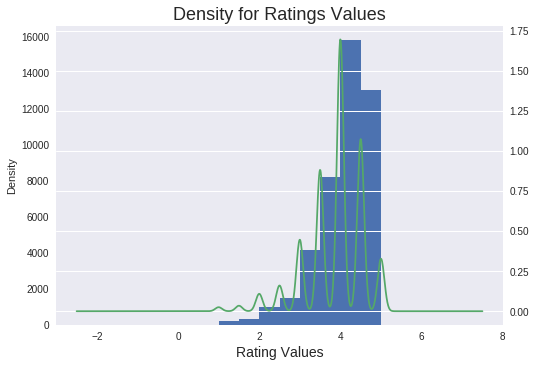
\includegraphics[scale=0.4]{density-ranting-values.png}
            \centering
            \caption{Density for user rating observations}
            % Figure reference: \ref{fig:fig-name}
            % Figure page reference:  \pageref{fig-name} 
            \label{fig:density-ranting-values}
        \end{figure}
        
        \item \textbf{Users}: The shape of the figure \ref{fig:user-density} is congruent with the tendency to have less users in the beginnig (the so-called early adopters) giving lots of ratings and helping the system to learn, and afterwads, a lot of new users giving a lot of less reviews. The same can be chequed out analogously for the items. We checked skewness ($skew=0.5$) and kurtosis($kurt=-0.9$) and confirmed bigger right tail and lack of outliers.
        
        \begin{figure}[h]
            
            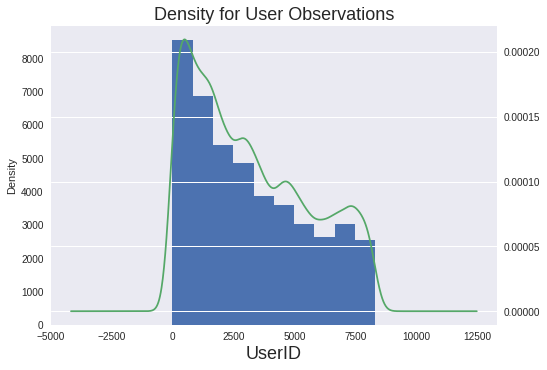
\includegraphics[scale=0.4]{userID_hist-kde.png}
            \centering
            \caption{Density for user rating observations}
            % Figure reference: \ref{fig:fig-name}
            % Figure page reference:  \pageref{fig-name} 
            \label{fig:user-density}
            
        \end{figure}
            
        \item \textbf{Items}:  It is interesting what the figure \ref{fig:item-density} shows. We can see a sort of different waves, characterized by a peak of ratings for some items, but a comparable bigger tail of items rated comparatively less. This may suggest that new items were introduced in 4 to 5 waves along time, where we initial introductions brought several more reviews per item introduced than the later, making sense with the previous analysis of users.
        
        \begin{figure}[h]
            
            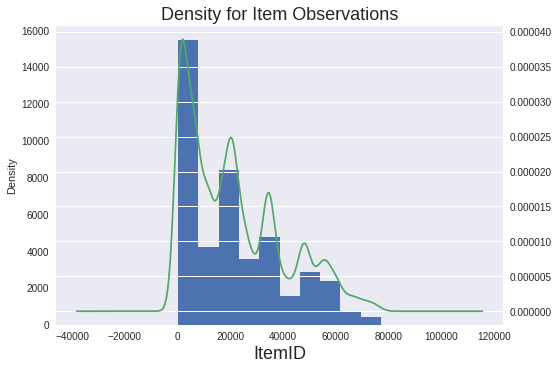
\includegraphics[scale=0.4]{ItemID_hist-kde.png}
            \centering
            \caption{Density for item rating observations}
            % Figure reference: \ref{fig:fig-name}
            % Figure page reference:  \pageref{fig-name} 
            \label{fig:item-density}
            
        \end{figure}
        
    \end{itemize}
    
        
    
    \item \textbf{Distribution}
    
    \begin{itemize}
        \item \textbf{User/Item}: we calculated the number of ratings per user. Table \ref{table:userid-itemid-description} shows a brief description of the data. The table is very informative, we can see that at least $25\%$ of the users have given just $1$ ranting, and that no more than $25\%$ of the users have given more than $5$ ratings. In average, users give $5$ ratings. The positive value for the skewness ($skew=5$) indicates that the right tail is bigger than the left, wich is consistent with our previous knowledge that there should be many users rating few items and much more less rating a lot. The kurtosis ($kurt=38.7$) high value is also consistent with this, showing the presence of outliers (users at the top of table). This can be clearly seen in the distribution figure below. Figure \ref{fig:userid-rating-frec} depicts this, although all this analysis relates userID with number of ratings, this tells us that the users with very few ratings are the ones with higher userID (maybe the ones that joined the system afterwards the early adopters), 
        
        \begin{figure}[h]
            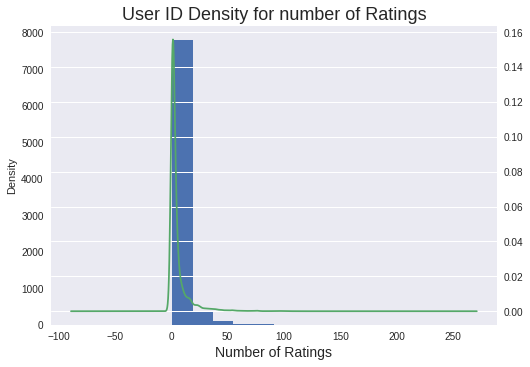
\includegraphics[scale=0.4]{userid-rating-frec.png}
            \centering
            \caption{Density for item rating observations}
            % Figure reference: \ref{fig:fig-name}
            % Figure page reference:  \pageref{fig-name} 
            \label{fig:userid-rating-frec}
        \end{figure}
        
        
        
        \begin{table}[]
        \centering
        \begin{tabular}{|>{\columncolor[HTML]{DAE8FC}}c|c|c|}
        \hline 
        \rowcolor[HTML]{DAE8FC} 
                    & UserID & userRatings   \\ \hline \hline
        count       & 8318      &  8318 \\ \hline
        mean        & 4159.91   &  5.33 \\ \hline
        std         & 2401.78   &  9.9  \\ \hline\hline
        min         & 1         & 1     \\ \hline
        25\%        & 2080      & 1     \\ \hline
        50\%        & 4159.5    & 2     \\ \hline
        75\%        & 6239      & 5     \\ \hline
        max\%        & 8320      & 181   \\ \hline\hline
        skewness    &   -  &  5.0   \\ \hline
        kurtosis    &   -  &  38.7  \\ \hline\hline
        
        
        \end{tabular}
        \caption{Description of user observations per userID}
        \label{table:userid-itemid-description}
        \end{table}
        
        We worked the data a little in order to explore how the distribution of number of ratings per user behaves. We got a positive value for the skewness ($skew=0.96$) indicates that the right tail is bigger than the left, which is consistent with our previous knowledge that there should be few users rating a lot of items and substantially more rating just a few. The kurtosis positive value ($kurt=1.67$) is also consistent with this, showing the presence of outliers (users at the top of table that are far away from the mean). This can be clearly seen in the distribution figure \ref{fig:ratings-per-user-density}.
        
        \begin{figure}[h]
            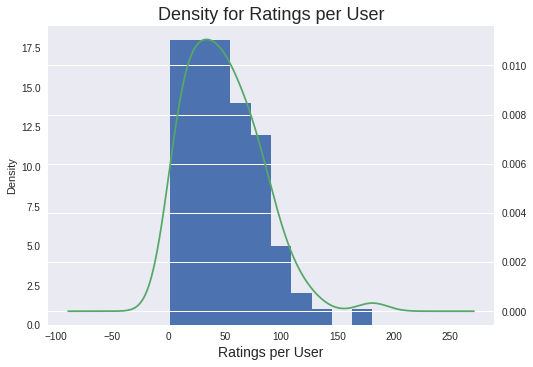
\includegraphics[scale=0.4]{ratings-per-user-density.png}
            \centering
            \caption{Distribution for user number of ratings}
            % Figure reference: \ref{fig:fig-name}
            % Figure page reference:  \pageref{fig-name} 
            \label{fig:ratings-per-user-density}
        \end{figure}
        
        
        
        \item \textbf{Item/User}: Making the same analysis as before for the rated items distribution, we worked the data to get the number of ratings per item. Table \ref{table:rating-observations-per-itemID} resumes the relevant information. We can see that at least $25\%$ of the items have been rated just once and that no more than $25\%$ of the items have been rated more than $7$ times. Items get approximately $24$ ratings In average. The positive value for the skewness ($skew=10.32$) indicates that the right tail is bigger than the left, which is consistent with our previous knowledge that there should be many items with few user ratings and much more less with a lot of rating. The kurtosis extreme high value ($kurt=136.46$) is also consistent with this, showing the presence of outliers (items at the top of table, we infer the most popular items). This can be clearly seen in the distribution figure \ref{fig:itemid-rating-frec}.
        
        
         \begin{figure}[h]
            
            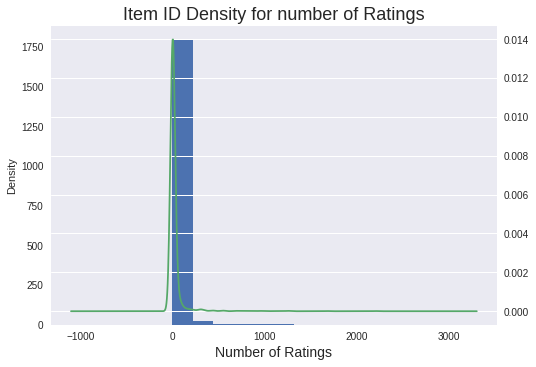
\includegraphics[scale=0.4]{itemid-rating-frec.png}
            \centering
            \caption{Distribution for user itemRatings}
            % Figure reference: \ref{fig:fig-name}
            % Figure page reference:  \pageref{fig-name} 
            \label{fig:itemid-rating-frec}
        \end{figure}
        
       
        \begin{table}[]
        \centering
        \begin{tabular}{|>{\columncolor[HTML]{DAE8FC}}c|c|c|}
        \hline 
        \rowcolor[HTML]{DAE8FC} 
                    & UserID & itemRatings   \\ \hline \hline
        count       & 1836      &  1836 \\ \hline
        mean        & 40.440    &  24   \\ \hline
        std         & 22.286    &  113  \\ \hline\hline
        min         & 175       & 1     \\ \hline
        25\%        & 21.640    & 1     \\ \hline
        50\%        & 41.525    & 2     \\ \hline
        75\%        & 60.511    & 7   \\ \hline
        max         & 77.207    & 2.205   \\ \hline\hline
        skewness    &  -   &  10.3   \\ \hline
        kurtosis    &   -  &  136.5  \\ \hline\hline
        
        
        \end{tabular}
        \caption{Description of rating observations per itemID}
        \label{table:rating-observations-per-itemID}
        \end{table}

        
        Although, same as before, the figure relates itemID with number of ratings, this tells us that the items with a lot of ratings are the ones with lower itemID (maybe the items that joined the system in the first stages and got much more time of exposure to user than the later ones), we worked the data to explore how the distribution of number of ratings per item behaves. We found that at least $25\%$ of the items have less than $40$ ratings and at most $25\%$ of the items hace more tan 230 ratings, on average items have aproximatelly $200$ ratings. The skewness ($skew=3.02$) indicates that the right tail is bigger than the left, wich is consistent with what we have discussed and the kurtosis ($kurt=11.14$) value reveals the presence of the Most Popular items outliers (items at the end of table that are far away from the mean). This can be clearly seen in the distribution figure \ref{fig:ratings-per-item-density}.
        
        \begin{figure}[h]
            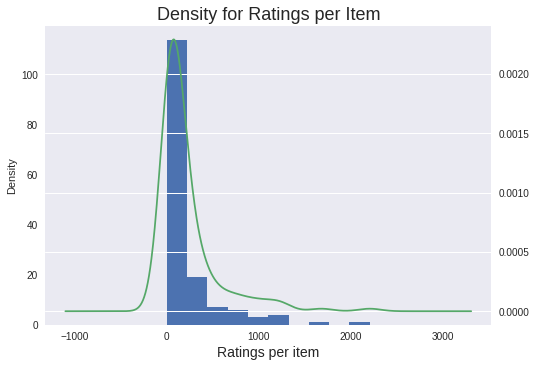
\includegraphics[scale=0.4]{ratings-per-item-density.png}
            \centering
            \caption{Distribution for item number of ratings}
            % Figure reference: \ref{fig:fig-name}
            % Figure page reference:  \pageref{fig-name} 
            \label{fig:ratings-per-item-density}
        \end{figure}
        
    \end{itemize}
    
\end{enumerate}

\section{Experimental Design}

In this section we present the experimental design selected. We describe the methods and the experimental plan to be performed.\\


\subsection{Methods}
\begin{enumerate}

    \item \textbf{UserKnn: } This algorithm interprets similar users as neighbors, if the user $n$ is similar to the user $u$, then $n$ is a neighbor of $u$. It generates a prediction for an item $i$ by analyzing the ratings for $i$ from the users in the neighborhood of $u$. Where:
    
    \begin{equation}
        pred(u,i)=\Bar{r}+ \frac{\displaystyle \sum_{n \subset N(u)}uSim(u,n)*(r_{ni}-\Bar{r}_{n})}{\displaystyle \sum_{n \subset N(u)}uSim(u,n)}
    \end{equation}
    
    Where $N(u)$ are the neighbors of $u$ and corresponds to the predicction for item $i$ that evaluates the ratings for $i$ from the neighbors of $u$. This formulation corrects for variations on the rating scale and weights it by each user' similarity to $u$ (the lower term corresponds to the result's normalization)
    
    A way to measure the similarity in this formulation is through Pearson Correlation:
    
    \begin{equation}
        uSim(u,n)= \frac{\displaystyle \sum_{i \subset CR(u,n)}(r_{ui}-\Bar{r}_{u})(r_{ni}-\Bar{r}_{n})}{ \displaystyle \sqrt{\displaystyle \sum_{i \subset CR_{(u,n)}}(r_{ui}-\Bar{r}_{u})^2}  \sqrt{\displaystyle \sum_{i \subset CR_{(u,n)}}(r_{ni}-\Bar{r}_{n})^2} }
    \end{equation}
    
    Where $CR_{(u, n)} $ are the coevaluated itemes between $ u $ and $ n $ and represents the similarity between the user $ u $ with user  $ n $ and $ \in [-1.0, 1.0] $, where $ 1.0 $ corresponds to a perfect similarity and $ -1.0 $ to its complement, in this context, we can choose only positive correlations to improve the prediction. This formulation analyzes similarities in ratings for items evaluated together with $ i $ (corrating).
    
    Although $UserKnn$ captures how recommendations are arranged and can detect complex patterns, as the data is sparce, it does not achieve general consensus regarding an item and pairs of users with few corratings are prone to throw biased correlations that can dominate the user's neighborhood in question.
    
    The algorithm can be implemented including all the users of the set as neighbors of each user, although by limiting it to the closest $k$ neighbors to each user improves its accuracy and efficiency. The challenge is to choose a well suited $k$ for the dataset. Even so, its implementation is expensive since it requires comparing each user with the complete set, so the time and memory for processing do not scale well as users and ratings increase. 
    
    
    \item \textbf{ItemKnn: } corresponds to the transpose of the previous problem, while user-based algorithms generate predictions based on similarities among users, the item-based does so based on similarities between items, that is, the prediction for an item is based on ratings for similar items. Thus, a prediction for a user $u$ of an item $i$ can be represented as the composition of weighted sums of ratings of the same user for the most similar items of $i$ 
    
    \begin{equation}
        pred(u,i)=\Bar{r}+ \frac{\displaystyle \sum_{n \subset RI(u)}iSim(i,j)*r_{ui}}{\displaystyle \sum_{n \subset RI(u)}iSim(i,j)}
    \end{equation}
    Where $RI(u)$ corresponds to the rated items by $u$.
    
    As the data on which the prediction is based upon all the data corresponding to the same user, it is not necessary to center the weighted sum as in the previous case. Analogously, $itemSim()$ corresponds to the measure of similarity between items i and j. The most popular and accurate similarity metric to calculate this similarity are pearson and the adjusted cosine that is shown below:
    
     \begin{equation}
        Corr(u,n)=\frac{\displaystyle \sum_{u \subset RB_{i,j}}(r_{ui}-\Bar{r}_{u})(r_{uj}-\Bar{r}_{u})}{ \sqrt{\displaystyle \sum_{u \subset RB_{i,j}}(r_{ui}-\Bar{r}_{u})^2}  \sqrt{\displaystyle \sum_{u \subset RB_{i,j}}(r_{uj}-\Bar{r}_{u})^2} }
    \end{equation}
    
    \begin{equation}
        CosSim(u,n)= 
        \frac{ \displaystyle\sum_{u \subset RB_{i,j}} r_{ui}*r_{uj} }
        {\displaystyle \sqrt{\sum_{u \subset RB_{i,j}}r_{ui}^2}
                        \sqrt{\sum_{u \subset RB_{i,j}}r_{uj}^2}}
    \end{equation}
    
    Where the set $RB_{i,j}$ corresponds to the set uf users who have rated $i$ and $j$ together. Although there is evidence that Itemknn is more accurate than UserKnn, in any case the size of the model grows quadratic on the number of items. There are different techniques to improve the use of memory, such as limiting the processing to $k$ corratings or retaining only the $n$ best correlations for each item (this may cause that the items correlated with the user's ratings do not contain the objective item)
    
    \item \textbf{SlopeOne: }
    This algorithm is based on the concept of deviation between items and users \cite{c7}, which item will like best a user than another.\\
    It is subtracted the average rating of the two items considered for the deviation, this is the deviation between the item j and the item k:
    \begin{equation}
        dev_{j,k} = \sum_{u_i\in I_{jk}} \frac{r_{ij}-r{ik}}{card(I_{jk})}
    \end{equation}
    where $I_{jk}$ is the user set with rated item $j$ and $k$.
    For the prediction of the unknown rating:
    \begin{equation}
        P(u)_j = \frac{\sum_{u_i\in I_{jk}}(dev_{j,k}+u_k)}{card(R_j)}
    \end{equation}
    where $R_j$ is the item set which are rated by the user.\\
    
    \item \textbf{SVD: }
    This algorithm consist in a matrix factorization technique, to reduce the number of features of the data set. The factorization is for the recommendation purpose.\\
    Each item is represented y a vector $q_i$ and each user by a vector $u_j$. The expected rating:
    \begin{equation}
        expected\_rating = q_i^Tu_j
    \end{equation}
    So, each vector can be found minimizing the square error difference, the difference between the known rating and the dot product:
    \begin{equation}
        minimum(u,q) \sum_{(j,i)\in K}(r_{ji}-q_i^Tu_j)^2
    \end{equation}
    \\
    
    \item \textbf{ALS: } 
    This algorithm works as an iterative optimization process. The idea is to arrive in each iteration to a closer factorized representation of our data.\\
    The original matrix R if dimension $u\times i$ where $u$ is the users and $i$ the items. We calculate a U and V matrices, that represent users and items hidden features, dimensions $u\times f$ and $f \times i$, f the number of features. The idea is that $R\approx U\times V$.\\
    Using least squares iteratively we can obtain the proper weights that describes the approximation of R.\\
    
\end{enumerate}

\subsection{Experiments}

Our experimental desing is implemented using \textit{Hold-Out}. We divide the data from the file \textit{training\_data.txt} in 2 parts, $70\%$ for training and $30\%$ for testing.\\
We adopt the \textit{Hold-Out} strategy taking into account the execution time and possibles drawbacks in the implementation. \textit{Cross-Validation} is a better strategy to obtain real metrics \cite{c6}, but to secure a successful work, we accept the trade-off favoring time over a more real metric.\\

\begin{enumerate}

    \item \textbf{UserKnn: }
    We increase the number of neighbour in 5, for each step. We start with 5 neighbours and we finish with 30 neighbours.
    
    \item \textbf{ItemKnn: } We follow the same strategy from \textit{UserKnn}. We start with 5 neighbours, increasing in 5 each step, until we arrived 30 neighbours.
    
    \item \textbf{SlopeOne: } This method does not requieres futher computation, there is no parameter tunning to perform.
    
    \item \textbf{SVD: } We change 2 parameters from this method, the number of factors and the iterations. We increment the number of factor in power of 10, from 10 to 1000. This plan is performed with 10 iterations and repeated with 200 iterations. 
    
    \item \textbf{ALS: } Following a similar strategy as in \textit{SVD}, we change 2 parameters from this method, the number of factors and the iterations. We increment the number of factor in 25, from 25 to 75. This plan is performed with 5 iterations and repeated with 15 iterations.
    
\end{enumerate}


\section{Results}

Here we present the results from the conducted experiments using \textit{UserKnn}, \textit{ItemKnn}, \textit{SlopeOne}, \textit{SVD} and \textit{ALS}.\\
We found that $k=30$ is the best parameter for \textit{UserKnn} (figure \ref{fig:MAE_UserKnn} and  \ref{fig:RMSE_UserKnn}). We observe in both curves, MAE and RMSE, as we increase the number of neighbours both metrics show better performance of the model.\\
We note the same behavior for \textit{ItemKnn}, we found the best parmeter is $k=30$ (figure \ref{fig:MAE_ItemKnn} and \ref{fig:RMSE_ItemKnn}). As we look at in MAE and RMSE curves, the performance of the model is best as we increase the number of neighbours.\\
In the case of \textit{SVD}, we observe the best combination of parameters is with $factor=1000$ and $iteration=100$ (figure \ref{fig:MAE_SVD} and \ref{fig:RMSE_SVD}). In both curves while we increase the number of factor the curves, MAE and RMSE, show better results. Also we can note that with less iteration the curve drops more. The curve with a 100 iterations works better than with 200 iterations.\\
We implement our experiments in \textit{Google Colab} with GPU. In terms of execution time, \textit{SlopeOne} is the model that takes less time $29.33 s$. The models that takes more excution time are \textit{ItemKnn} and \textit{UserKnn} with $1115.21 s$ and $3270.64 s$ respectively (table \ref{exctime-data}). With GPU the execution time improves considerably, in particular on those models that required more time.\\
We note that the model with better performance is \textit{SVD}. We compare RMSE and nDCG in \textit{UserKnn}, \textit{ItemKnn} and \textit{SlopeOne}, the three models behave very similar. The major diferences between those models are in the nDCG metric (table \ref{raw-data}).\\

\begin{table}[]
\centering
\begin{tabular}{|c|c|c|c|c|c|}
\hline 
\rowcolor[HTML]{DAE8FC} 
Algorithm & parameters & MAE & RMSE & MAP@10 & nDCG@10   \\ \hline \hline
UserKnn   & k=30  &  0.5014 &  0.6572   & 0.0014 & 0.0010 \\ \hline
ItemKnn   & k=30  &  0.4919 &  0.6586 &  0.0058 & 0.0073  \\ \hline
SlopeOne   & -  &   0.4841 &  0.6471   &   0.0002   &  0.0002 \\ \hline

SVD   & f=1000-it=100  & 0.4536 &  0.6020   &   0.0178   & 0.0107  \\ \hline
\dots       &        &         &        &          &            \\ \hline
ALS   & -   & -     & -    &    -   & - \\ \hline

\end{tabular}
\caption{Results}
\label{raw-data}
\end{table}

\begin{table}[]
\centering
\begin{tabular}{|c|c|}
\hline 
\rowcolor[HTML]{DAE8FC} 
Algorithm & Execution time [s]   \\ \hline \hline
UserKnn   & 3270.64  \\ \hline
ItemKnn   & 1115.21  \\ \hline
SlopeOne  & 29.33  \\ \hline
SVD       & 53.62  \\ \hline
\dots     &   \\ \hline
ALS       &  - \\ \hline

\end{tabular}
\caption{Execution Time}
\label{exctime-data}
\end{table}

\begin{figure}[h]
            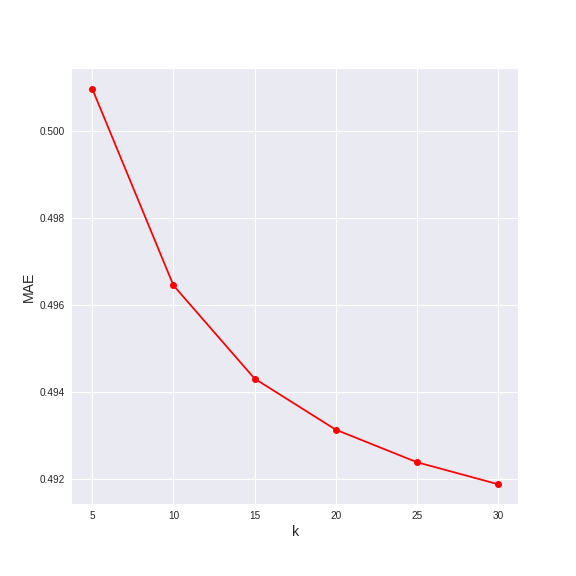
\includegraphics[scale=0.4]{MAE_itemKnn.png}
            \centering
            \caption{MAE plot for ItemKnn}
            \label{fig:MAE_ItemKnn}
        \end{figure}
 \begin{figure}[h]
            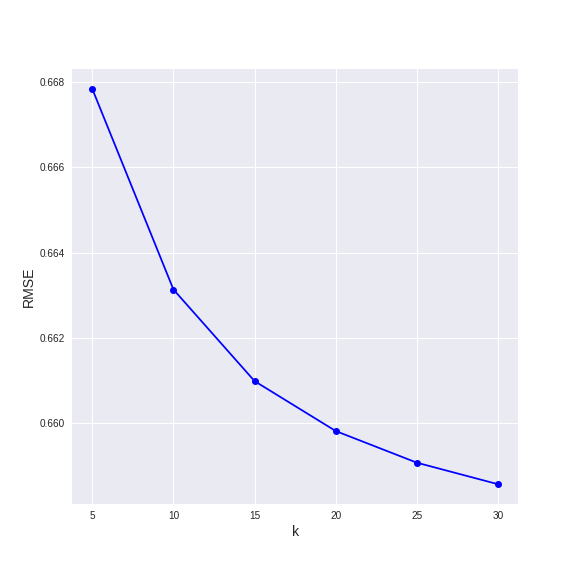
\includegraphics[scale=0.4]{RMSE_itemKnn.png}
            \centering
            \caption{RMSE plot for ItemKnn}
            \label{fig:RMSE_ItemKnn}
        \end{figure}       

\begin{figure}[h]
            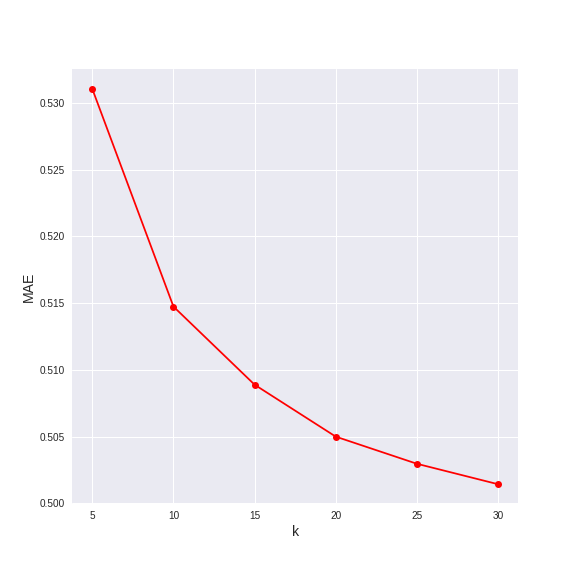
\includegraphics[scale=0.4]{MAE_userKnn.png}
            \centering
            \caption{MAE plot for UserKnn}
            \label{fig:MAE_UserKnn}
        \end{figure}
 \begin{figure}[h]
            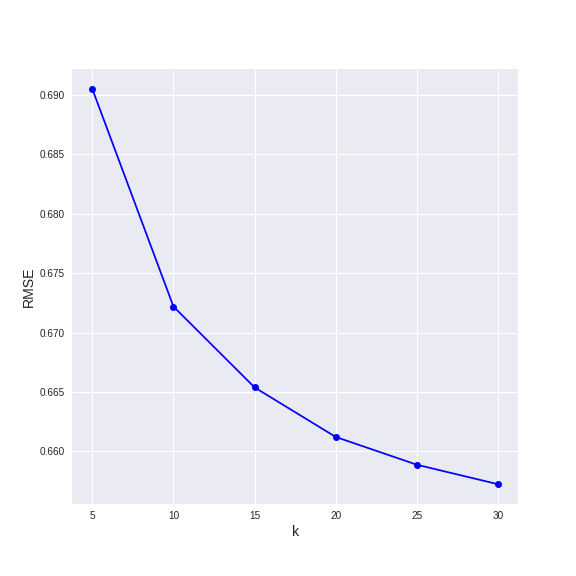
\includegraphics[scale=0.4]{RMSE_userKnn.png}
            \centering
            \caption{RMSE plot for UserKnn}
            \label{fig:RMSE_UserKnn}
        \end{figure} 

\begin{figure}[h]
            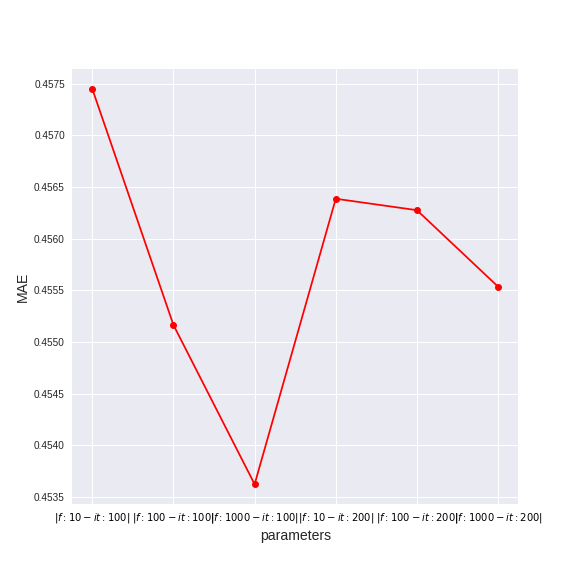
\includegraphics[scale=0.4]{MAE_SVD.png}
            \centering
            \caption{MAE plot for SVD}
            \label{fig:MAE_SVD}
        \end{figure}
 \begin{figure}[h]
            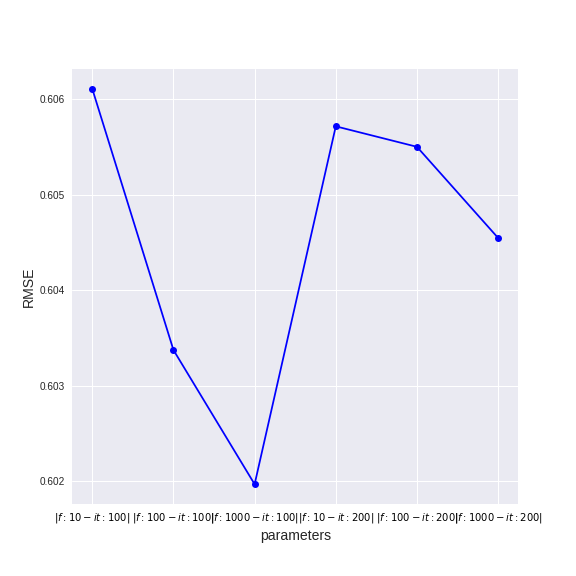
\includegraphics[scale=0.4]{RMSE_SVD.png}
            \centering
            \caption{RMSE plot for SVD}
            \label{fig:RMSE_SVD}
        \end{figure}

\section{Discussion}
%\section{Sensitivity Analysis}

In this section we discuss and analyze the effect the different model parameters have on the results.\\

\begin{enumerate}
    \item Item Knn: figure \ref{fig:item_knn-param-analysis} depicts the MAE and RMSE progression according to different neighbor carnality. It is pretty straightforward to notice to see that it has an inverted U-shape relationship, the optimal (minimum error) can be found at approximately 30 neighbors.
    
    \begin{figure}[h]
        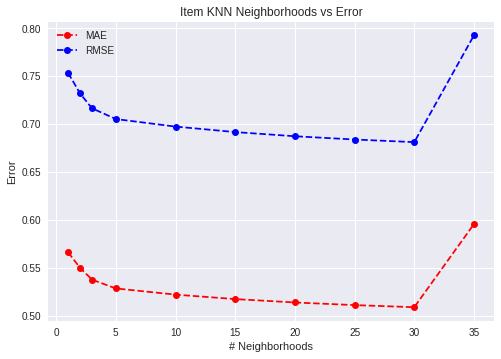
\includegraphics[scale=0.4]{item_knn-param-analysis.png}
        \centering
        \caption{MAE and RMSE Error against item KNN Neighborhoods}
        % Figure reference: \ref{fig:fig-name}
        % Figure page reference:  \pageref{fig-name} 
        \label{fig:item_knn-param-analysis}
    \end{figure}
        
    \item User Knn: figure \ref{fig:user_knn-param-analysis} also shows MAE and RMSE progression according to different neighbor carnality. The effect of increasing the number of neighbors it is marginal over the error. We had to set an improvement threshold of $0.01$ to stop the descent, otherwise, the algorithm keeps kinding that adding one neighbor improves the error. That lead us to the asymptotic bound of $0.492$ for $MAE$ and $0.649$ for $RMSE$ with $100$ neighbors, beyond those bounds, the error improvement of the model is unsignificant. But we can see relatively no improvement from $20$ neighbors and forth, training more would only mean more cpu, memory and time expense with relatively no improvement. 
    
\begin{figure}[h]
        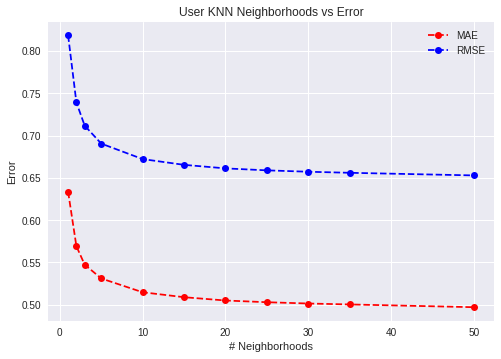
\includegraphics[scale=0.4]{user_knn-param-analysis.png}
        \centering
        \caption{MAE and RMSE Error against user KNN Neighborhoods}
        % Figure reference: \ref{fig:fig-name}
        % Figure page reference:  \pageref{fig-name} 
        \label{fig:user_knn-param-analysis}
    \end{figure}
    
    \item SVD
    
    \begin{itemize}
        \item Factor analysis: same as with userKnn, he had to set an improvement threshold per iteration of $0.001$ decrement on error to stop the descent. Having that done, the minimal $MAE$ and $RMSE$ found was $0.455$ with $150$ factors and $0.602$ with $200$ factors. Figure \ref{fig:SVD-param-analysis} shows MAE and RMSE progression according to increasing factor cardinality.
    
        \begin{figure}[h]
            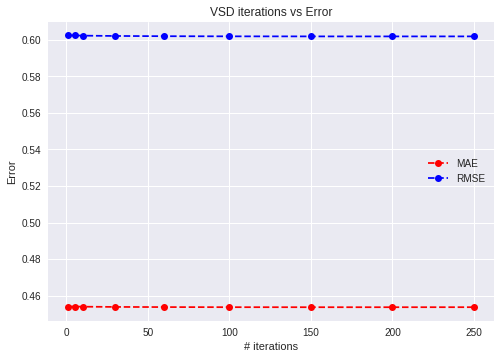
\includegraphics[scale=0.4]{SVD-param-analysis.png}
            \centering
            \caption{MAE and RMSE Error against number of factors}
            % Figure reference: \ref{fig:fig-name}
            % Figure page reference:  \pageref{fig-name} 
            \label{fig:SVD-param-analysis}
        \end{figure}
        
        \item Iterations analysis: we has a similar situation for the iterations parameter. The error descent was so marginal that the progression plot looked exactly as Figure \ref{fig:SVD-param-analysis} just shown. The minimal $MAE$ and $RMSE$ found was $0.454$ with $150$ max-iterations and $0.601$ with $200$ max-iterations.
        
    \end{itemize}
    
\end{enumerate}

\section{Conclusion}

In this work we test several recommendation algorithms for a beer selling platform. The data analysis section allowed us to get a more profound comprehension of the inherent complexities of the used data. We found out the data indeed suffer from dimensionality issues like many items with poor rating frequency and only a couple with exorbitantly high number of ratings.  We infer those items are the most popular ones. The case of users was less extreme, in the case that the user that had a higher rating frequency were no so outliered than the rest. The mean ratings per user was much higher than for the item case. This has a direct impact on the algorithm performance, placing \textit{UserKnn} has more neighbors better positioned at ranking task than \textit{ItemKnn}, but reporting worst performance on error measurements. Even so, \textit{SVD} beats them all on error and ranking performance. Also in terms of execution time, \textit{SVD} presents a very good time compared to \textit{ItemKnn} and \textit{UserKnn}.\\
So for the task of generate recommendation, we choose \textit{SVD} method over all others to pursue the objective of recommend beers in the \textit{Pybeerlab} plataform.




\addtolength{\textheight}{-12cm}   % This command serves to balance the column lengths
                                  % on the last page of the document manually. It shortens
                                  % the textheight of the last page by a suitable amount.
                                  % This command does not take effect until the next page
                                  % so it should come on the page before the last. Make
                                  % sure that you do not shorten the textheight too much.


\begin{thebibliography}{99}

\bibitem{c1} Schafer, J. B., Frankowski, D., Herlocker, J., & Sen, S. (2007). Collaborative filtering recommender systems. In The adaptive web (pp. 291-324). Springer Berlin Heidelberg.

\bibitem{c2} How not to sort by Average Rating, Evan Miller Blog

\bibitem{c3} Koren, Y., Bell, R., & Volinsky, C. (2009). Matrix factorization techniques for recommender systems. Computer IEEE Magazine, 42(8), 30–37.

\bibitem{c4} Hu, Y., Koren, Y., & Volinsky, C. (2008, December). Collaborative filtering for implicit feedback datasets. In Data Mining, 2008. ICDM’08. Eighth IEEE International Conference on (pp. 263–272). IEEE.


\bibitem{c5} L. Van der Maaten and G. Hinton. Visualizing data using t-sne. Journal of Machine Learning Research, 9(2579-2605):85, 2008.

\bibitem{c6} Sanjay Y. and Sanyam S. Analysis of k-Fold Cross-Validation over Hold-Out Validation on Colossal Datasets for Quality Classification. IEEE 6th International Conference on Advanced Computing (IACC), 2016.

\bibitem{c7} Jingjiao L., Limei S. and Jiao W. A Slope One Collaborative Filtering Recommendation Algorithm Using Uncertain Neighbors Optimizing. Lecture Notes in Computer Science book series, volume 7142, pp 160-166, 2011.






\end{thebibliography}




\end{document}
